\documentclass[12pt]{article}
\usepackage[margin=1in]{geometry}
\usepackage{color}
\usepackage{graphicx}
\title{Comments on creating a mesh}
\author{Peter Monk}
\begin{document}
\maketitle

\section{Introduction}
This document is not intended as a tutorial on meshing in {\tt NGSpy}.  My intention is to describe some of the assumptions made in the code.  The scatterer (or scatterers) must be contained in a circle centered at the origin 
of radius \verb+pml_rad+ and the annular PML has thickness \verb+pml_delta+.  The choice of these parameters depends on the wavenumber $\kappa$ and is discussed a little more in \verb+helmholtz_penetrable.ipynb+.  See Fig.~\ref{fig1}.
\begin{figure}[h]
\begin{center}
\resizebox{0.5\textwidth}{!}{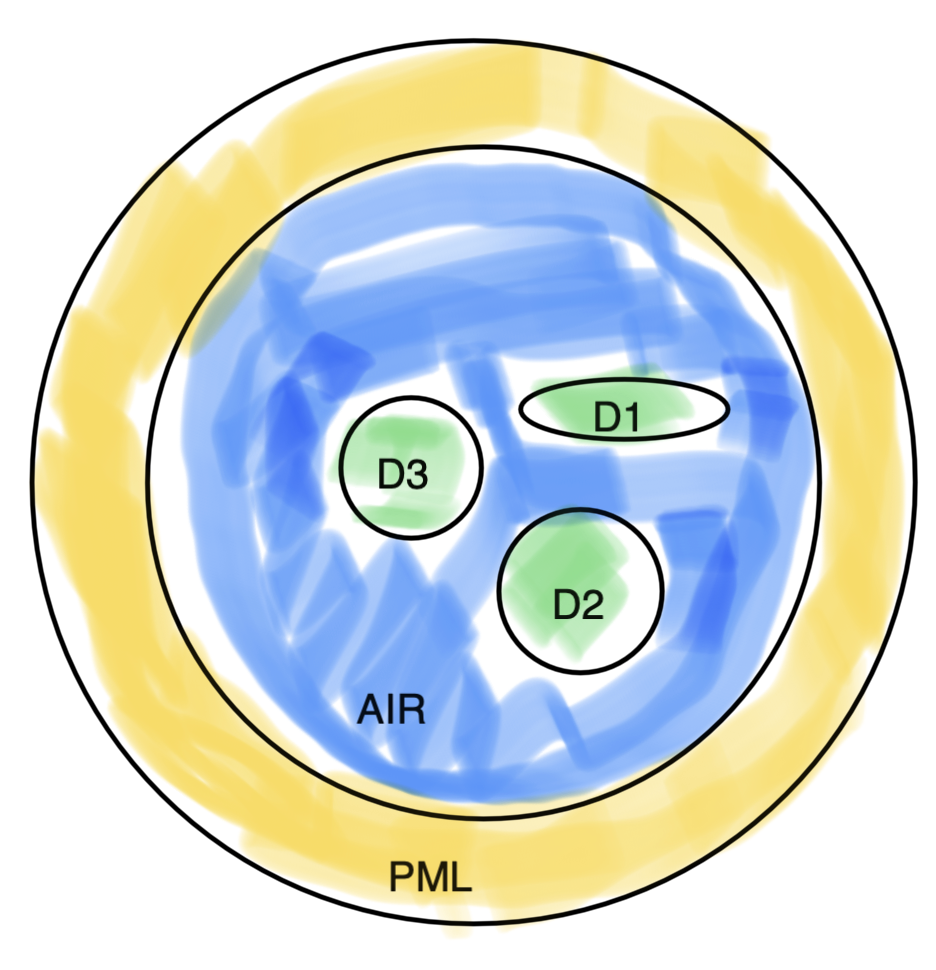
\includegraphics{domain.png}}
\end{center}
\caption{Some components of the computational domain. D1, D2 etc are components of the scatterer.}\label{fig1}
\end{figure}
\section{Example: a penetrable square}
Here is the code for square scatterer centered at the origin.  Note that I use keyword arguments to set
parameters.  This makes it easy to set defaults that give a nice picture as I develop a mesh for 
a new scatterer.  But these \textcolor{red}{must be reset when you use the meshing file} to be the actual values 
needed for the simulation (saying again: the values here are to get a nice picture of the geometry, not an accurate scattering solution).
\begin{verbatim}
def square(hmax_s=0.1,hmax_a=0.1,pml_rad=2,pml_delta=.8,order=3):
    geo = SplineGeometry()
    geo.AddCircle( (0,0), pml_rad+pml_delta, leftdomain=2, bc="outerbnd")
    geo.AddCircle( (0,0), pml_rad, leftdomain=1, rightdomain=2)
    
    # start code for square
    L2=1/2
    p1,p2,p3,p4 = [ geo.AppendPoint(x,y) for x,y in [ (-L2,-L2), (L2,-L2),
                                                           (L2,L2),(-L2,L2)]]
    geo.Append (["line", p1, p2],leftdomain=3,rightdomain=1,bc="scatterer")
    geo.Append (["line", p2, p3],leftdomain=3,rightdomain=1,bc="scatterer")
    geo.Append (["line", p3, p4],leftdomain=3,rightdomain=1,bc="scatterer")
    geo.Append (["line", p4, p1],leftdomain=3,rightdomain=1,bc="scatterer")
    geo.SetMaterial(3,'D')
    geo.SetDomainMaxH(3,hmax_s)
    # end code for square
    
    geo.SetMaterial(1, "air")
    geo.SetMaterial(2, "pmlregion")
    geo.SetDomainMaxH(1,hmax_a)
    geo.SetDomainMaxH(2,hmax_a)
    # genenerate an NGSpy mesh
    mesh = Mesh(geo.GenerateMesh(maxh=hmax_a))
    mesh.Curve(order) # The PML boundaries are curved.
    return(mesh)
\end{verbatim}
Lets discuss section by section:
\begin{verbatim}
def square(hmax_s=0.1,hmax_a=0.1,pml_rad=2,pml_delta=.8,order=3):
    geo = SplineGeometry()
    geo.AddCircle( (0,0), pml_rad+pml_delta, leftdomain=2, bc="outerbnd")
    geo.AddCircle( (0,0), pml_rad, leftdomain=1, rightdomain=2)
\end{verbatim}
The arguments \verb+hmax_s+ and \verb+hmax_a+ are used to set the requested mesh size in the 
scatterer or air/PML respectively.  I have made no attempt to refine the mesh near corners.
The arguments \verb+pml_rad+ and \verb+pml_delta+ set the inner radius and thickness of the PML. The \verb+order+ parameter will ultimately be the polynomial degree of the FEM.  I should, I guess, have supplied the edge length of the square as a parameter, but didn't bother.  Note that the PML is region with index 2 and ``air'' is region 1.  The outer boundary of the PML must be labelled \verb+outerbound+.

Next comes the specific code to define the scatterer:
\begin{verbatim}
    # start code for square
    L2=1/2
    p1,p2,p3,p4 = [ geo.AppendPoint(x,y) for x,y in [ (-L2,-L2), (L2,-L2),
                                                           (L2,L2),(-L2,L2)]]
    geo.Append (["line", p1, p2],leftdomain=3,rightdomain=1,bc="scatterer")
    geo.Append (["line", p2, p3],leftdomain=3,rightdomain=1,bc="scatterer")
    geo.Append (["line", p3, p4],leftdomain=3,rightdomain=1,bc="scatterer")
    geo.Append (["line", p4, p1],leftdomain=3,rightdomain=1,bc="scatterer")
    geo.SetMaterial(3,'D')
    geo.SetDomainMaxH(3,hmax_s)
    # end code for square
\end{verbatim}
The scatterer can be multiply connected.  Each component needs an index (here 3). The outer boundary of each component must be labelled \verb+scatterer+ and \textcolor{red}{must be traced anti-clockwise.} The latter requirement is to ensure the correct orientation of normals. and is critical for a correct far field calculation. Use \verb+SetMaterial+ to give a name to each component to be used in the scattering code, and set the mesh size to \verb+hmax_s+ so we can refine inside a scatterer.

Now we complete by giving a nme \verb+pmlregion" to the PML and \verb+air+ to the exterior of the scatterer.  Also set the mesh size here to \verb+hmax_a+ and then generate the mesh.  Finally curve the mesh.
\begin{verbatim}
    geo.SetMaterial(1, "air")
    geo.SetMaterial(2, "pmlregion")
    geo.SetDomainMaxH(1,hmax_a)
    geo.SetDomainMaxH(2,hmax_a)
    # genenerate an NGSpy mesh
    mesh = Mesh(geo.GenerateMesh(maxh=hmax_a))
    mesh.Curve(order) # The PML boundaries are curved.
    return(mesh)
\end{verbatim}
\section{Example: two impenetrable squares}
This example is from \verb+geometries_dirichlet.py+ and meshes outside a triangle. The triangle can both be rotated by an angle \verb+ang+ radians and be translated by \verb+xcen+.  The variable \verb+angle+ sets one angle of an isosceles triangle.  The main points are that 1) the outer boundary of the (possibly disconnected) scatterer is labeled \verb+dirichlet+ and 2) the boundaries of the
components of the scatterer need to be traversed anti-clockwise.  
\begin{verbatim}
def triangle(hmax=0.1,pml_rad=2.,pml_width=.8,R=1,xcen=(0,0),
                 ang=0,angle=np.pi/8):
    geo = SplineGeometry()
    geo.AddCircle( (0,0), pml_rad+pml_width, leftdomain=2, bc="outerbnd")
    geo.AddCircle( (0,0), pml_rad, leftdomain=1, rightdomain=2)
    ###
    mat=np.array([[np.cos(ang),np.sin(ang)],[-np.sin(ang),np.cos(ang)]])
    X1=np.matmul(mat,np.array([-R,0]))+xcen;
    X2=np.matmul(mat,np.array([R*np.cos(angle),R*np.sin(angle)]))+xcen;
    X3=np.matmul(mat,np.array([R*np.cos(angle),-R*np.sin(angle)]))+xcen;
    p1,p2,p3 = [ geo.AppendPoint(x,y) for x,y in [X1, X2, X3]]
    geo.Append (["line", p1, p3],leftdomain=0,rightdomain=1,bc="dirichlet",
                    maxh=hmax/2)
    geo.Append (["line", p3, p2],leftdomain=0,rightdomain=1,bc="dirichlet",
                    maxh=hmax/2)
    geo.Append (["line", p2, p1],leftdomain=0,rightdomain=1,bc="dirichlet",
                    maxh=hmax/2)
    ###
    geo.SetMaterial(1, "air")
    geo.SetMaterial(2, "pmlregion")
    mesh = Mesh(geo.GenerateMesh(maxh=hmax))
    return(mesh)    
   \end{verbatim}
   The mesh-size is now set in the domain and somewhat smaller along the edges. Obviously the inside of the triangle is not meshed.
\end{document}
